\documentclass{article}

% if you need to pass options to natbib, use, e.g.:
% \PassOptionsToPackage{numbers, compress}{natbib}
% before loading nips_2016
%
% to avoid loading the natbib package, add option nonatbib:
% \usepackage[nonatbib]{nips_2016}

\usepackage[final]{nips_style}
\usepackage[utf8]{inputenc} % allow utf-8 input
\usepackage[T1]{fontenc}    % use 8-bit T1 fonts
\usepackage{hyperref}       % hyperlinks
\usepackage{url}            % simple URL typesetting
\usepackage{booktabs}       % professional-quality tables
\usepackage{amsfonts}       % blackboard math symbols
\usepackage{nicefrac}       % compact symbols for 1/2, etc.
\usepackage{microtype}      % microtypography

\usepackage{amsmath}
\usepackage{latexsym}
\usepackage{graphicx}
\usepackage{amssymb}
\usepackage{mathtools}
\usepackage{bm}
\usepackage{listings}
\usepackage{subfig}
\usepackage{array}
\usepackage{multirow}
\usepackage{float}
\usepackage{subfig}

\DeclareMathOperator*{\argmax}{\arg\max}
\DeclareMathOperator*{\argmin}{\arg\min}

\newcommand{\diag}[0]{\operatorname{diag}}
\newcommand{\vect}[1]{\mathbf{#1}}
\newcommand{\vects}[1]{\boldsymbol{#1}}
\newcommand{\matr}[1]{\mathbf{#1}}
\newcommand{\matrs}[1]{\boldsymbol{#1}}

\newcommand{\va}[0]{\vect{a}}
\newcommand{\vb}[0]{\vect{b}}
\newcommand{\vc}[0]{\vect{c}}
\newcommand{\vd}[0]{\vect{d}}
\newcommand{\ve}[0]{\vect{e}}
\newcommand{\vf}[0]{\vect{f}}
\newcommand{\vg}[0]{\vect{g}}
\newcommand{\vh}[0]{\vect{h}}
\newcommand{\vi}[0]{\vect{i}}
\newcommand{\vj}[0]{\vect{j}}
\newcommand{\vk}[0]{\vect{k}}
\newcommand{\vl}[0]{\vect{l}}
\newcommand{\vm}[0]{\vect{m}}
\newcommand{\vn}[0]{\vect{n}}
\newcommand{\vo}[0]{\vect{o}}
\newcommand{\vp}[0]{\vect{p}}
\newcommand{\vq}[0]{\vect{q}}
\newcommand{\vr}[0]{\vect{r}}
\newcommand{\vs}[0]{\vect{s}}
\newcommand{\vt}[0]{\vect{t}}
\newcommand{\vu}[0]{\vect{u}}
\newcommand{\vv}[0]{\vect{v}}
\newcommand{\vw}[0]{\vect{w}}
\newcommand{\vx}[0]{\vect{x}}
\newcommand{\vy}[0]{\vect{y}}
\newcommand{\vz}[0]{\vect{z}}
\newcommand{\valpha}[0]{\vects{\alpha}}
\newcommand{\vtheta}[0]{\vects{\theta}}
\newcommand{\veta}[0]{\vects{\eta}}
\newcommand{\vmu}[0]{\vects{\mu}}

\newcommand{\mA}[0]{\matr{A}}
\newcommand{\mB}[0]{\matr{B}}
\newcommand{\mC}[0]{\matr{C}}
\newcommand{\mD}[0]{\matr{D}}
\newcommand{\mE}[0]{\matr{E}}
\newcommand{\mF}[0]{\matr{F}}
\newcommand{\mG}[0]{\matr{G}}
\newcommand{\mH}[0]{\matr{H}}
\newcommand{\mI}[0]{\matr{I}}
\newcommand{\mJ}[0]{\matr{J}}
\newcommand{\mK}[0]{\matr{K}}
\newcommand{\mL}[0]{\matr{L}}
\newcommand{\mM}[0]{\matr{M}}
\newcommand{\mN}[0]{\matr{N}}
\newcommand{\mO}[0]{\matr{O}}
\newcommand{\mP}[0]{\matr{P}}
\newcommand{\mQ}[0]{\matr{Q}}
\newcommand{\mR}[0]{\matr{R}}
\newcommand{\mS}[0]{\matr{S}}
\newcommand{\mT}[0]{\matr{T}}
\newcommand{\mU}[0]{\matr{U}}
\newcommand{\mV}[0]{\matr{V}}
\newcommand{\mW}[0]{\matr{W}}
\newcommand{\mX}[0]{\matr{X}}
\newcommand{\mY}[0]{\matr{Y}}
\newcommand{\mZ}[0]{\matr{Z}}
\newcommand{\mSigma}[0]{\matrs{\Sigma}}

\DeclareMathOperator*{\E}{E}
\DeclareMathOperator*{\tr}{tr}
\DeclareMathOperator*{\prox}{prox}
\DeclareMathOperator*{\conv}{conv}
\DeclareMathOperator*{\minimize}{minimize}
\DeclareMathOperator*{\maximize}{maximize}
\DeclareMathOperator*{\sign}{sign}
\DeclareMathOperator*{\vecop}{vec}
\DeclareMathOperator*{\Poisson}{Poisson}
\DeclareMathOperator*{\Cat}{Cat}
\DeclareMathOperator*{\Dir}{Dir}
\DeclareMathOperator*{\Exp}{Exp}
\DeclareMathOperator*{\DiscreteUniform}{DiscreteUniform}
\newcommand{\R}{\mathbb{R}}

\DeclarePairedDelimiter{\abs}{\lvert}{\rvert}
\DeclarePairedDelimiter{\norm}{\lVert}{\rVert}
\DeclarePairedDelimiter{\inprod}{\langle}{\rangle}
\DeclarePairedDelimiter{\floor}{\lfloor}{\rfloor}

\newcommand{\AND}{\wedge}
\newcommand{\OR}{\vee}

\lstset{frame=tb,
  aboveskip=3mm,
  belowskip=3mm,
  showstringspaces=false,
  columns=flexible,
  basicstyle={\small\ttfamily},
  numbers=none,
  breaklines=true,
  breakatwhitespace=true,
  tabsize=4
}

\allowdisplaybreaks

\renewcommand{\thesubsection}{\thesection \,\,(\alph{subsection})}
\renewcommand{\thesubsubsection}{\thesection \,\,(\alph{subsection})\,\,[\roman{subsubsection}]
                                 }

\bibliographystyle{abbrvnat}

\title{Monte Carlo Methods: Homework 3}

\author{
  Prithvi Krishna Gattamaneni\\
  \texttt{pkg238@nyu.edu} \\
}
%xxxxxxxxxxxxxxxxxxxxxxxxxxxxxxxxxxxxxxxxxxxxxxxxxxxxxxxxxxxxxxxxxxxxxxxxxxxxxx%

\begin{document}

\maketitle

\section{Fake Data Creation} %%1
For the creation of fake data, the following values were chosen. The base case values are chosen as shown in the table below. The values of t were chosen uniformly between 0 and 10. The number of datapoints varies as per the experiment, but for the base case this number is 1000.\\
\begin{center}
	\begin{tabular}{ |c| c| }
		\hline
		Parameter & Value\\
		\hline
		m & 2 \\ 
		A & [0.2, 0.8] \\  
		$\lambda$ & [0.4, 0.6]\\
		sigma & 0.3 \\
		N & 1000\\
		\hline
	\end{tabular}
\end{center}


\section{Likelihood Function} %%2
\[
L(\theta) = \prod_{i=1}^{N} \frac{1}{\sqrt{2\pi\sigma^2}}\exp\left( \frac{(Y_i - f(t_i;\theta))^2}{2\sigma^2} \right)
\]
Here $\theta$ is the set of parameters involving the components of A and lambda.


\section{Procedure for MCMC step} %%3
Assuming the current set of parameters is $\theta_t$, and that the new proposed set of parameters is $\theta^*$.
\\
For a single step in this algorithm, it is possible to make a Gaussian isotropic proposal for both A and lambda, and a Gaussian proposal for sigma. However in order to make a better proposal I used a Gaussian multivariate isotropic proposal, that uses as mean the current set of parameters in the chain. This new proposal is $\theta^*$. The transition probability matrix in this case is symmetric as well. 
For calculating the prior probability, I use an uninformative prior that assumes that both A and lambda components are between 0 and 1. This prior probability $P(\theta)$ returns 0 if the parameters are outside of this range and returns 1 otherwise\\
\[
\pi(\theta^*) = P(\theta^*).L(\theta^*)
\]
\[
\pi(\theta^t) = P(\theta^t).L(\theta^t)
\]
The acceptance probability $A(\theta_t, \theta^*)$ is
\[
A(\theta_t, \theta^*) = \frac{\pi(\theta^*)}{\pi(\theta^t)}
\]
if $A(\theta_t, \theta^*)$ is more than one I accept $\theta^*$ else I accept $\theta^*$ only with probablity $A(\theta_t, \theta^*)$.

\newpage
\section{MH Experiments} %%4

\subsection{Base Case} %%4a
In this section the metropolis hastings algorithm is run for a long time to collect more than a million samples from the posterior in each experiment. Shown below are the scatter plots for the parameters A, lambda and sigma. Also shown are the sample values in sequence for the first component of A and lambda. Note that the actual values are represented by two points on the scatter plots. This is because an inversion between the components of A and $\lambda$ is an equivalent solution.

\begin{figure}[H]
	\centerline{\subfloat[$A_0$]{{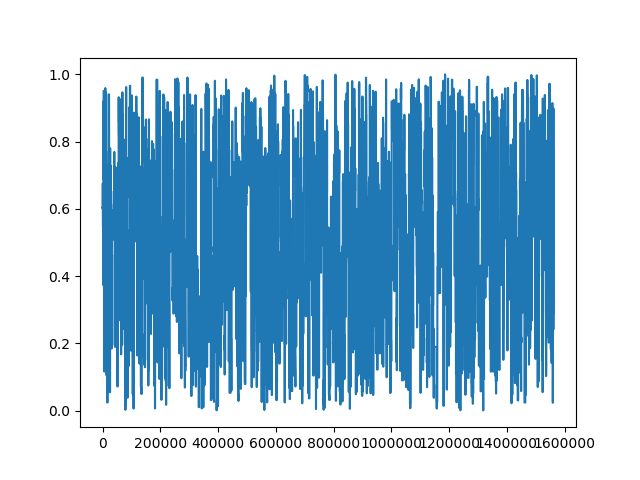
\includegraphics[scale=0.65]{graphs/r1_A_seq0} }}
		\subfloat[$\lambda_0$]{{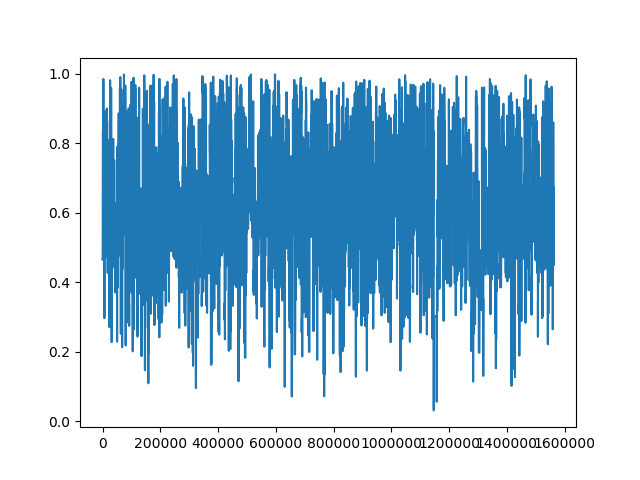
\includegraphics[scale=0.65]{graphs/r1_L_seq0} }}}
	\caption{Values of first components of A and lambda as each sample is generated}
	\label{1.fig:r1_seq}
\end{figure}

\newpage
\begin{figure}[H]
	\centerline{\subfloat[$A$]{{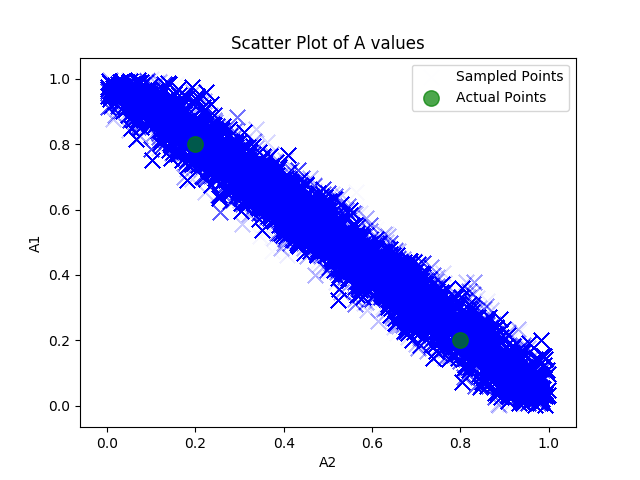
\includegraphics[scale=0.65]{graphs/r1_AScatter} }}
		\subfloat[$\lambda$]{{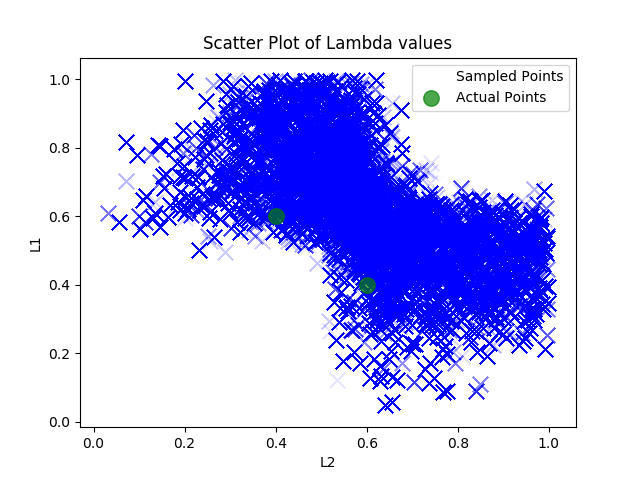
\includegraphics[scale=0.65]{graphs/r1_LScatter} }}}
	\caption{Scatter plot showing the distribution of values that are sampled for both A and lambda.}
	\label{1.fig:r1_scat}
\end{figure}

\begin{figure}[H]
	\centerline{\subfloat[$\sigma$]{{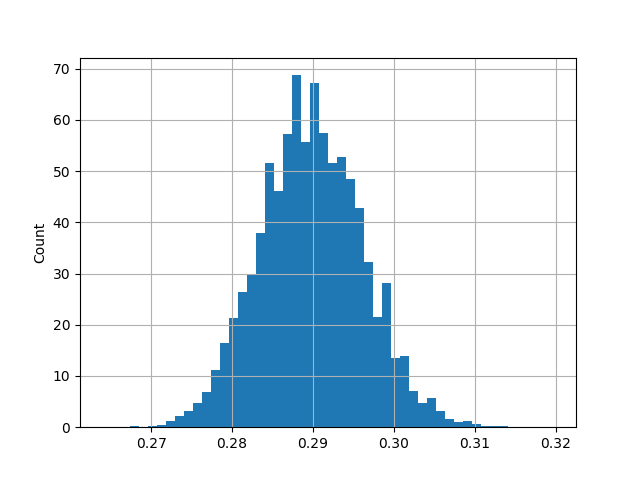
\includegraphics[scale=0.65]{graphs/r1_Sigma} }}}
	\caption{Histogram showing most sampled sigma values.}
	\label{1.fig:r1_sigma}
\end{figure}

From the above figures we see that the distribution of parameters that could generate this data seems quite broad and does cover the actual values that were used to generate the data. The values of sigma that were most sampled seem to be close to the actual value of sigma which is 0.3. On calculating the auto correlation time for each variable I find that it is around 3000 for the components of both A and $\lambda$


\subsection{Increasing the number of datapoints} %%4b
In this section we keep the rest of the parameters the same except that the number of datapoints is now increased from 1000. We try to show that as we increase the number of datapoints the distribution of solutions that can generate this dataset should become sparser and verify it with the help of scatter plots.\\

\subsubsection{Number of datapoints = 5000} %%4b
Here we increase the value of N from 1000 to 5000 and observe the differences.
Shown below are the scatterplots for the sampled values for both A and lambda. We see that the distribution of values is now more sparse than before. Also looking at the sequence of values that is generated we see that it is harder to generate a new sample and the progress of the samples is less diverse.

\begin{figure}[H]
	\centerline{\subfloat[N=1000]{{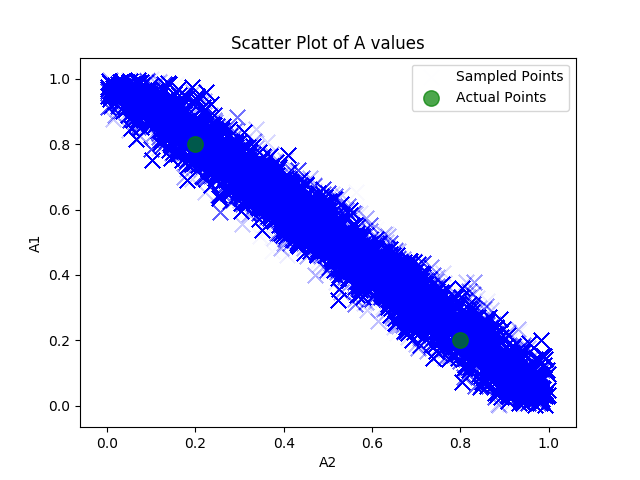
\includegraphics[scale=0.65]{graphs/r1_AScatter} }}
		\subfloat[N=5000]{{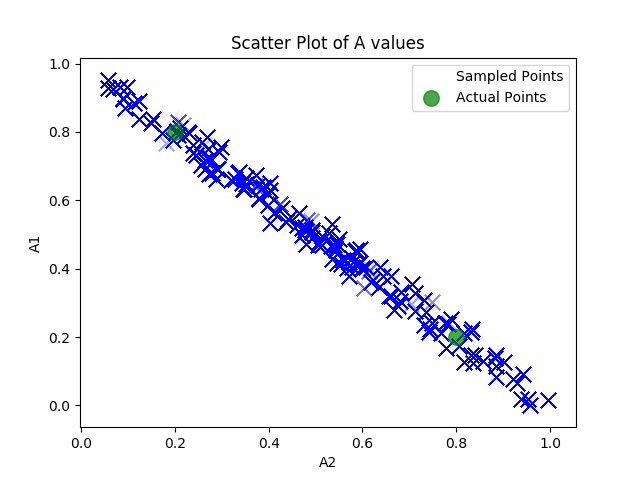
\includegraphics[scale=0.65]{graphs/r2_AScatter} }}}
	\caption{Scatter plot showing the distribution of values that are sampled for A.}
	\label{1.fig:r2_scat_A}
\end{figure}

\newpage
\begin{figure}[H]
	\centerline{\subfloat[N=1000]{{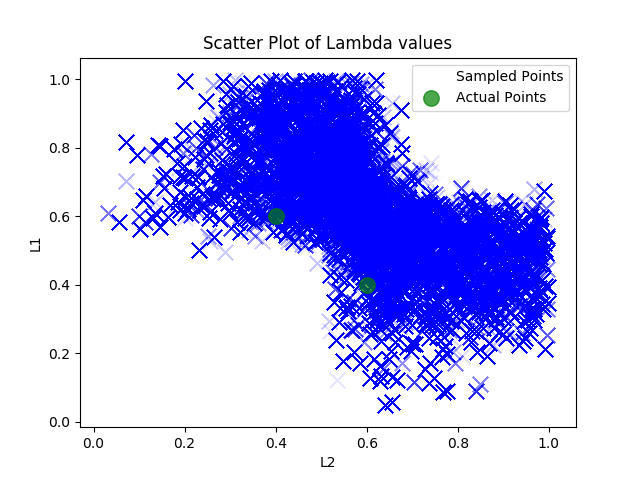
\includegraphics[scale=0.65]{graphs/r1_LScatter} }}
		\subfloat[N=5000]{{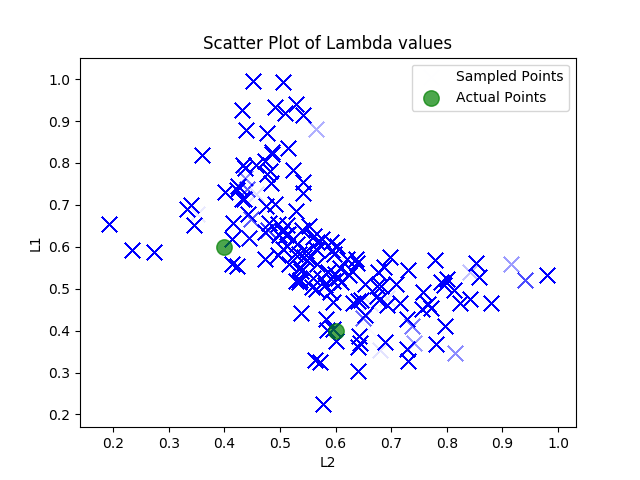
\includegraphics[scale=0.65]{graphs/r2_LScatter} }}}
	\caption{Scatter plot showing the distribution of values that are sampled for $\lambda$.}
	\label{1.fig:r2_scat_L}
\end{figure}

\begin{figure}[H]
	\centerline{\subfloat[$A_0$]{{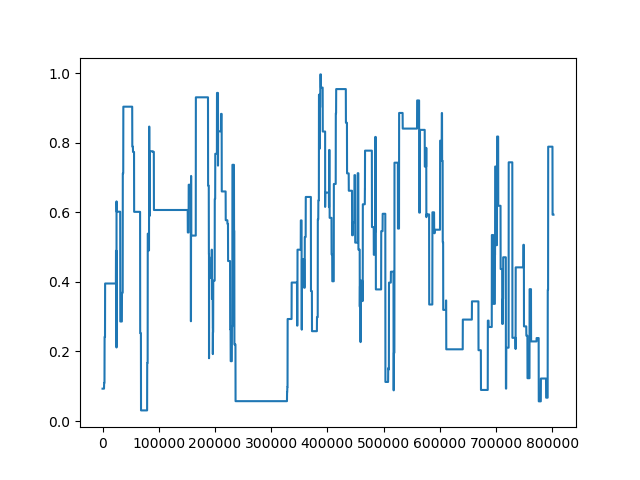
\includegraphics[scale=0.65]{graphs/r2_A_seq0} }}
		\subfloat[$\lambda_0$]{{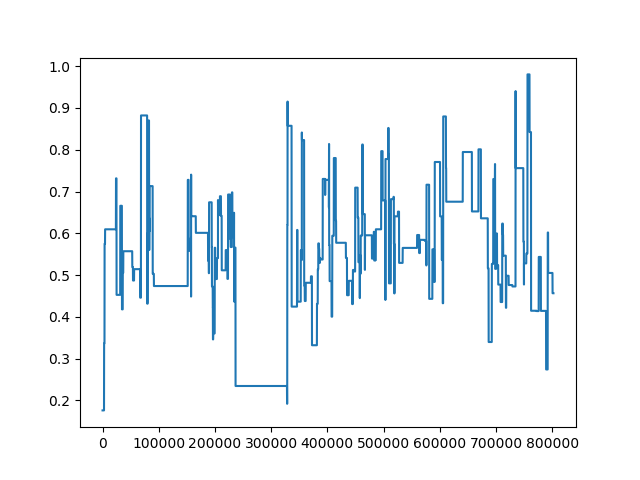
\includegraphics[scale=0.65]{graphs/r2_L_seq0} }}}
	\caption{Values of first components of A and lambda as each sample is generated. N=5000}
	\label{1.fig:r2_seq}
\end{figure}

\subsubsection{Number of datapoints = 10000} %%4b
Here we increase the value of N from 5000 to 10000 and observe the differences.
Shown below are the scatterplots for the sampled values for both A and lambda. We see that the distribution of values is now even more sparse than before. 

\begin{figure}[H]
	\centerline{\subfloat[N=5000]{{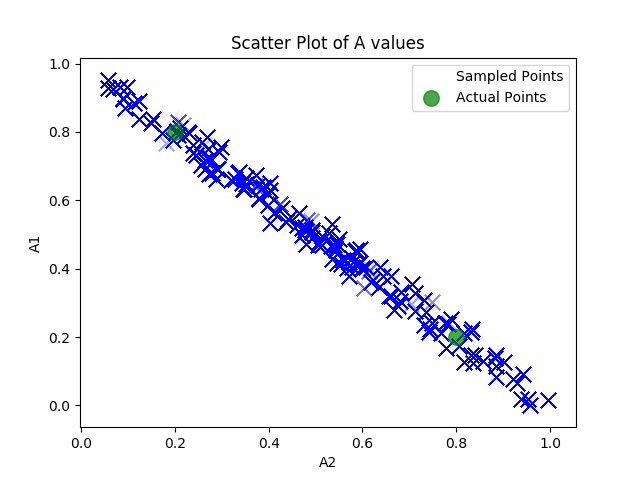
\includegraphics[scale=0.65]{graphs/r2_AScatter} }}
		\subfloat[N=10000]{{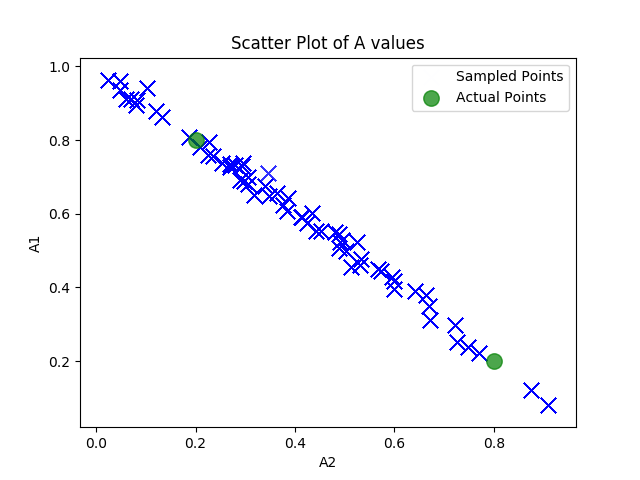
\includegraphics[scale=0.65]{graphs/r3_AScatter} }}}
	\caption{Scatter plot showing the distribution of values that are sampled for A.}
	\label{1.fig:r3_scat_A}
\end{figure}

\begin{figure}[H]
	\centerline{\subfloat[N=5000]{{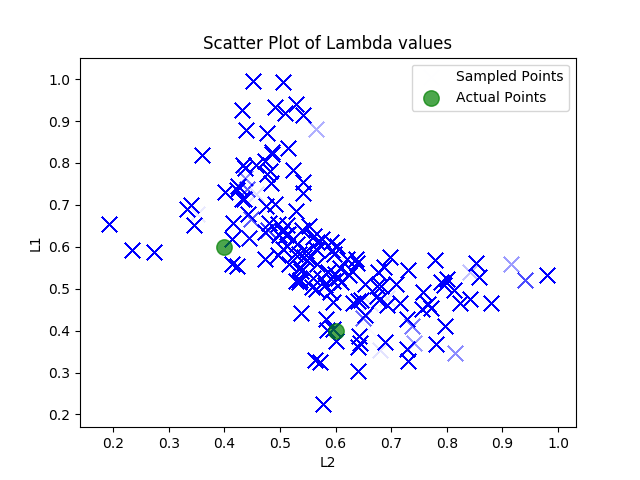
\includegraphics[scale=0.65]{graphs/r2_LScatter} }}
		\subfloat[N=10000]{{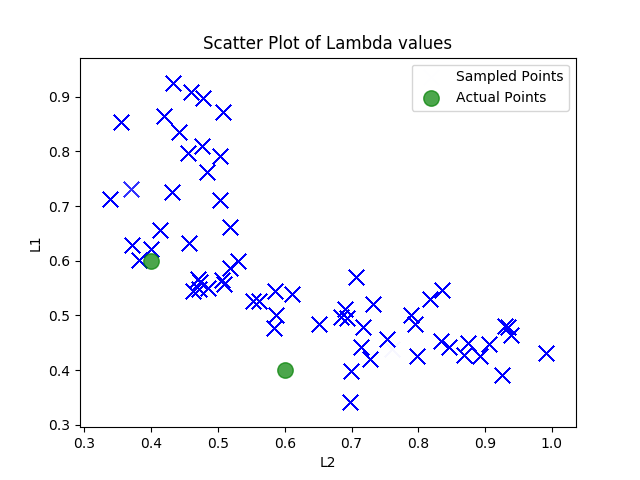
\includegraphics[scale=0.65]{graphs/r3_LScatter} }}}
	\caption{Scatter plot showing the distribution of values that are sampled for $\lambda$.}
	\label{1.fig:r3_scat_L}
\end{figure}

\begin{figure}[H]
	\centerline{\subfloat[$A_0$]{{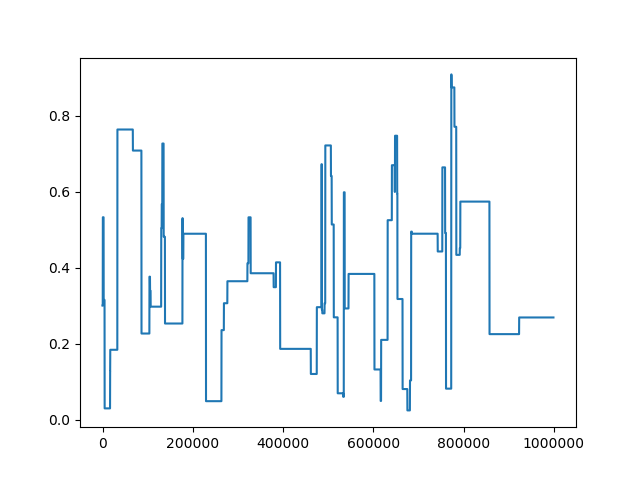
\includegraphics[scale=0.65]{graphs/r3_A_seq0} }}
		\subfloat[$\lambda_0$]{{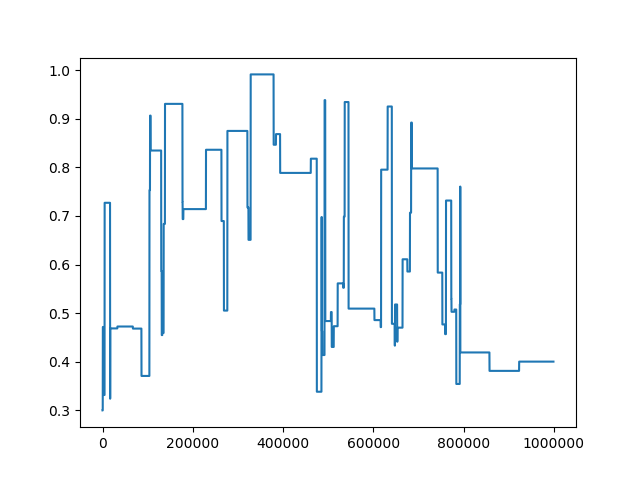
\includegraphics[scale=0.65]{graphs/r3_L_seq0} }}}
	\caption{Values of first components of A and lambda as each sample is generated. N=10000}
	\label{1.fig:r3_seq}
\end{figure}
We observe that the distribution of parameters generated by the sampler has now gotten even more sparse. This shows that as the dataset size increases the solution becomes more sparse and converges to the actual datapoint values.

\newpage
\subsection{Increasing the proposal width} %%4b
In this section we keep all the parameters the same except that the proposal width of the new sample is now increased in the gaussian proposal from 0.1 to 0.3. We try to show that as we increase the proposal width the distribution of solutions that can generate this dataset should become sparser and verify it with the help of scatter plots.\\

\begin{figure}[H]
	\centerline{\subfloat[N=5000 r=0.1]{{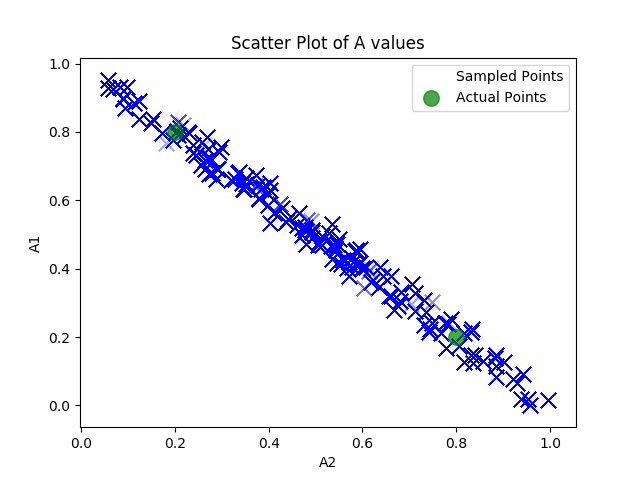
\includegraphics[scale=0.65]{graphs/r2_AScatter} }}
		\subfloat[N=10000 r=0.3]{{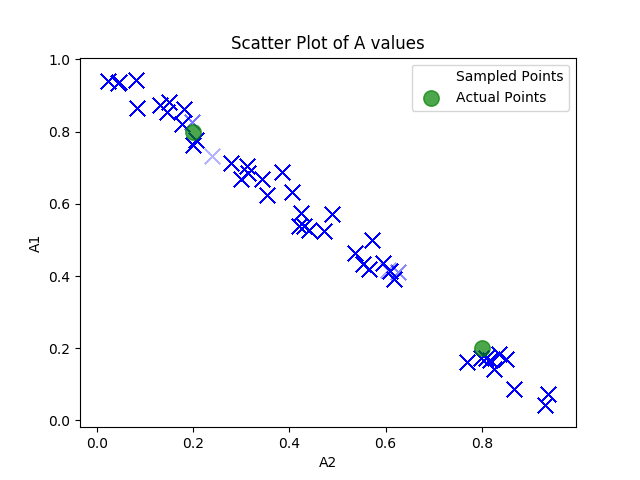
\includegraphics[scale=0.65]{graphs/r4_AScatter} }}}
	\caption{Scatter plot showing the distribution of values that are sampled for A.}
	\label{1.fig:r5_scat_A}
\end{figure}

\begin{figure}[H]
	\centerline{\subfloat[N=5000 r=0.1]{{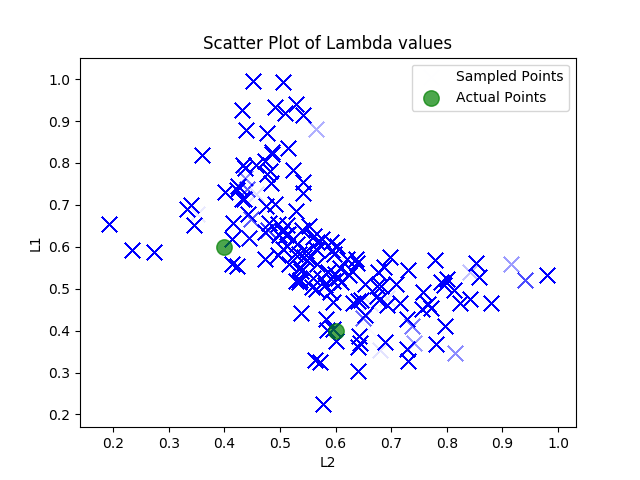
\includegraphics[scale=0.65]{graphs/r2_LScatter} }}
		\subfloat[N=5000 r=0.3]{{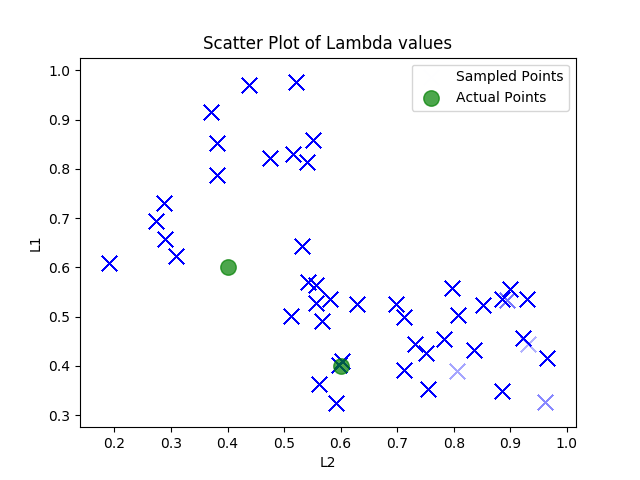
\includegraphics[scale=0.65]{graphs/r4_LScatter} }}}
	\caption{Scatter plot showing the distribution of values that are sampled for $\lambda$.}
	\label{1.fig:r5_scat_L}
\end{figure}

The above plots show that when the proposal width r (length scale) increases the distribution becomes sparse and converges to the actual solution.


\begin{figure}[H]
	\centerline{\subfloat[$A_0$]{{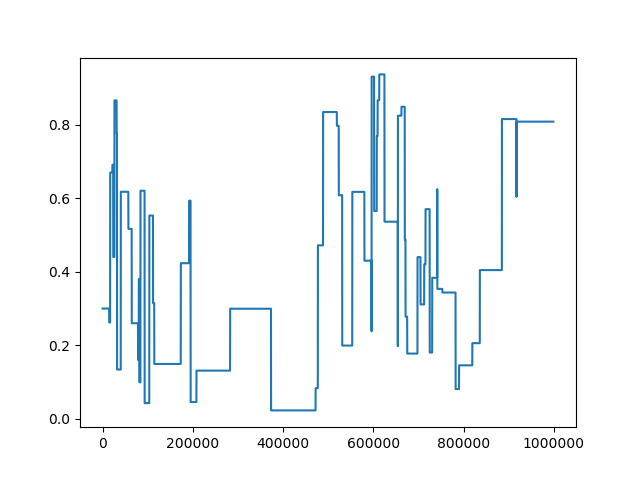
\includegraphics[scale=0.65]{graphs/r4_A_seq0} }}
		\subfloat[$\lambda_0$]{{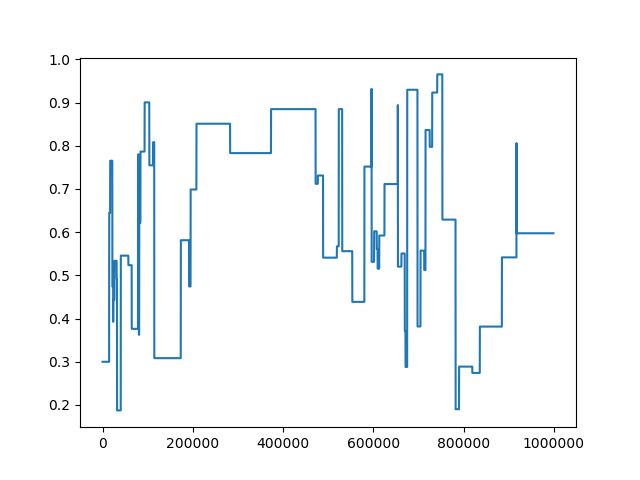
\includegraphics[scale=0.65]{graphs/r4_L_seq0} }}}
	\caption{Values of first components of A and lambda as each sample is generated. N=10000}
	\label{1.fig:r5_seq}
\end{figure}

\newpage
\begin{lstlisting}[language=Python]
--------create_fake_data.py----------------
import numpy as np
import json

def create_fake_data(use_default=True):
    param_file = open('params.json')
    params = json.load(param_file)

    m = params["m"]
    sigma = params["sigma"]
    N = params["N"]

    A_vals = []
    lambda_vals = []
    if use_default==False:
        #need to sample m A's and m lambdas
        A_vals = np.random.uniform(0,1,m)
        #lambda_vals = np.random.randint(1, N/2, size=m)
        lambda_vals = np.random.uniform(0, 1, size=m)

        np.savetxt(params["A_file"], A_vals )
        np.savetxt(params["lambda_file"], lambda_vals)
    else:
        A_vals = np.loadtxt(params["A_file"])
        lambda_vals = np.loadtxt(params["lambda_file"])

    data = []
    #times = np.arange(0, 1, 1.0/ N)
    times = np.arange(0, 10.0, 10.0 / N)
    #times = np.random.uniform(low=0.0, high=1.0, size=N)

    for t in times:
        l2 = lambda_vals * t * -1
        e = np.exp(l2)
        datapoint = np.dot(A_vals,e)
        data.append(datapoint)

    data = np.array(data)
    data = data + sigma * np.random.normal(0,1,N)

    np.savetxt(params["Y_file"], data)
    np.savetxt(params["times_file"], times)


if __name__ == "__main__":
    create_fake_data()
--------------------------------------
------hw2_funcs.py--------------------
import numpy as np
import scipy.stats
import json
import math
import time

#This function returns a vector, which is f(t) for each t in times
def eval_f(A_vals, lambda_vals, times, m):
    l1 = np.reshape(lambda_vals, (m, 1))
    c = l1 * times
    c = np.exp(-1 * c)
    r = np.dot(A_vals, c)
    return r

def eval_likelihood(A_vals, lambda_vals, times, data_points, m, sigma):
    r = eval_f(A_vals, lambda_vals, times, m)
    val = ((r - data_points)*(r - data_points)) / (2 * sigma )
    val = np.exp(-1 * val)
    t = 1.0
    for item in val:
        t = t * item
    return t

def eval_log_likelihood(A_vals, lambda_vals, times, data_points, m, sigma):
    r = eval_f(A_vals, lambda_vals, times, m)
    val = ((r - data_points)*(r - data_points)) / (2 * sigma * sigma )
    val = np.exp(-1 * val)
    norm = math.sqrt(2 * math.pi * sigma * sigma)
    val = val / norm
    val = np.log(val)
    t = 0.0
    for item in val:
        t = t + item
    return t

def eval_prior_prob_log_sum(A_vals, lambda_vals, sigma):
    return np.log(eval_prior_prob(A_vals, lambda_vals, sigma))

def eval_prior_prob(A_vals, lambda_vals, sigma):
    if sigma < 0 or sigma > 1:
        return 0
    for i in range(0,len(A_vals)):
        if A_vals[i] < 0 or A_vals[i] > 1:
            return 0
        if lambda_vals[i] < 0 or lambda_vals[i] > 1:
            return 0
    return 1.0 * eval_prior_prob_sigma(sigma)

def eval_prior_prob_sigma(sigma):
    param_file = open('params.json')
    params = json.load(param_file)
    mean = params["sigma"]
    return scipy.stats.norm(mean, 0.1).pdf(sigma)

def propose_new_A(A, m):
    A_new = np.random.multivariate_normal(A, 0.1 * np.identity(m))
    return A_new

def propose_new_lambda(lambda_old, m):
    lambda_new = np.random.multivariate_normal(lambda_old, 0.1 * np.identity(m))
    return lambda_new

def propose_new_sigma(sigma_old):
    return np.random.normal(sigma_old, 0.05)

def MCMC_MH(Y, times, m):
    A = 0.5 * np.ones(m)
    lambdas = 0.5 * np.ones(m)
    A = np.array([0.3, 0.7])
    lambdas = np.array([0.3, 0.7])

    param_file = open('params.json')
    params = json.load(param_file)
    sigma = params["sigma"]
    num_iter = params["num_iter"]
    time_iter = params["time_iter"]

    i = 0
    A_history = []
    L_history = []
    sigma_history = []
    likelihood_history = []


    t_end = time.time() + 60 * time_iter
    #while time.time() < t_end:
    while i < num_iter:
        A_new = propose_new_A(A, m)
        lambda_new = propose_new_lambda(lambdas, m)
        sigma_new = propose_new_sigma(sigma)

        prior_old = eval_prior_prob_log_sum(A, lambdas, sigma)
        likelihood_old = eval_log_likelihood(A, lambdas, times, Y, m, sigma)

        prior_new = eval_prior_prob_log_sum(A_new, lambda_new, sigma_new)
        likelihood_new = eval_log_likelihood(A_new, lambda_new, times, Y, m, sigma_new)

        logp = likelihood_new + prior_new - (likelihood_old + prior_old)
        if logp > 0:
            A = A_new
            lambdas = lambda_new
            sigma = sigma_new
            likelihood_history.append(likelihood_new)
            print ("found new sample ", i)
        else:
            prob = np.exp(logp)
            sample = np.random.uniform(0,1)
            if sample < prob:
                A = A_new
                lambdas = lambda_new
                sigma = sigma_new
                #i += 1
                print ("found new sample with prob", i)
                print (sample, prob)
                likelihood_history.append(likelihood_new)
            else:
                likelihood_history.append(likelihood_old)


        A_history.append(A)
        L_history.append(lambdas)
        sigma_history.append(sigma)
        i += 1

    print("NumIter is ", i)
    np.savetxt("L_result", np.array(L_history))
    np.savetxt("A_result", np.array(A_history))
    np.savetxt("sigma_result", np.array(sigma_history))
    np.savetxt("likelihood_result", np.array(likelihood_history))


if __name__ == "__main__":
    param_file = open('params.json')
    params = json.load(param_file)
    Y = np.loadtxt(params["Y_file"])
    m = params["m"]
    times = np.loadtxt(params["times_file"])
    MCMC_MH(Y, times, m)
-----------------------------------------------
------graph_plot.py----------------------------
import numpy as np
import json
import matplotlib.pyplot as plt

def plotGraph(x, name):
    n, bins, patches = plt.hist(x, normed=1, bins=50)
    plt.ylabel('Count')
    plt.grid(True)
    plt.savefig(name)
    plt.clf()

def plotGraphs():
    Y = np.loadtxt("A_result")
    val = Y[:, 0:1]
    val = val.tolist()
    plotGraph(val)

def plotGraphsA():
    param_file = open('params.json')
    params = json.load(param_file)
    Y = np.loadtxt("A_result")
    m = params["m"]
    for i in range(0,m):
        val = Y[1000:,i:i+1]
        name = "A" + str(i)
        plotGraph(val, name)

def plotGraphsL():
    param_file = open('params.json')
    params = json.load(param_file)
    Y = np.loadtxt("L_result")
    m = params["m"]
    for i in range(0,m):
        val = Y[1000:,i:i+1]
        name = "L" + str(i)
        plotGraph(val, name)

def plotGraphsSigma():
    param_file = open('params.json')
    params = json.load(param_file)
    Y = np.loadtxt("sigma_result")
    m = params["m"]
    name = "Sigma"
    plotGraph(Y, name)

def plotSeq():
    param_file = open('params.json')
    params = json.load(param_file)
    m = params["m"]
    for i in range(0,m):
        Y = np.loadtxt("A_result")
        plt.plot(range(len(Y)-1000), Y[1000:, i])
        plt.savefig("A_seq" + str(i))
        plt.clf()
    for i in range(0, m):
        Y = np.loadtxt("L_result")
        plt.plot(range(len(Y)-1000), Y[1000:, i])
        plt.savefig("L_seq" + str(i))
        plt.clf()

def plotScatterA():
    #lt.figure(figsize=(10, 8))
    param_file = open('params.json')
    params = json.load(param_file)
    Y = np.loadtxt("A_result")
    m = params["m"]
    A = np.loadtxt(params["A_file"])
    val1 = Y[100000:, 0:0 + 1]
    val2 = Y[100000:, 1:1 + 1]

    plt.scatter(val1, val2, marker='x', color='b', alpha=0.0021,
                s=124,label='Sampled Points')
    plt.scatter([A[0], A[1]], [A[1], A[0]], marker='o', color='g', alpha=0.7,
                s=124, label='Actual Points')
    # Chart title
    plt.title('Scatter Plot of A values')
    plt.ylabel('A1')
    plt.xlabel('A2')
    plt.legend(loc='upper right')
    plt.savefig("AScatter")
    plt.clf()


def plotScatterLambda():
    #lt.figure(figsize=(10, 8))
    param_file = open('params.json')
    params = json.load(param_file)
    Y = np.loadtxt("L_result")
    m = params["m"]
    A = np.loadtxt(params["lambda_file"])
    val1 = Y[100000:, 0:0 + 1]
    val2 = Y[100000:, 1:1 + 1]

    plt.scatter(val1, val2, marker='x', color='b', alpha=0.0021,
                s=124,label='Sampled Points')
    plt.scatter([A[0], A[1]], [A[1], A[0]], marker='o', color='g', alpha=0.7,
                s=124, label='Actual Points')


    # Chart title
    plt.title('Scatter Plot of Lambda values')
    plt.ylabel('L1')
    plt.xlabel('L2')
    plt.legend(loc='upper right')
    plt.savefig("LScatter")
    plt.clf()


def plotGraphs():
    plotGraphsA()
    plt.clf()

    plotGraphsL()
    plt.clf()

    plotGraphsSigma()
    plt.clf()

    plotSeq()
    plt.clf()

    plotScatterA()
    plotScatterLambda()


if __name__ == "__main__":
    plotGraphs()

-----------------------------------------------
------statistics.py----------------------------
import numpy as np
import json
import matplotlib.pyplot as plt

def getmean(series):
    return np.mean(series, axis=0)

def autocorrelation_fn(series,mean):
    n = len(series)
    T = int(np.ceil(n/2))
    cov = np.correlate(series-mean, series-mean, mode = 'same')
    C = cov[-T:]
    C /= n -1 - np.arange(T)
    rho = np.array(C)
    for t in range(T):
        rho[t] = C[t]/C[0]
    return rho,C

def autcorrelation_time(rho, window=5):
    tau = 1
    t = 1
    while(window*tau > t and t <len(rho)):
        tau += rho[t]
        t += 1
    return tau


def calculateStats():
    param_file = open('params.json')
    params = json.load(param_file)
    A = np.loadtxt("A_result")
    L = np.loadtxt("L_result")
    m = params["m"]
    acts = []
    print ("Here1")
    for i in range(0,m):
        print ("Here2")
        rhoA,CA = autocorrelation_fn(A[:,i], getmean(A[:,i]))
        act = autcorrelation_time(rhoA)
        acts.append(act)
        plt.plot(range(0,len(rhoA)), rhoA)
        plt.savefig("Aauto" + str(i))
        plt.clf()
    for i in range(0,m):
        print ("Here3")
        rhoL,CL = autocorrelation_fn(L[:,i], getmean(L[:,i]))
        act = autcorrelation_time(rhoL)
        acts.append(act)
        plt.plot(range(0, len(rhoL)), rhoL)
        plt.savefig("Lauto" + str(i))
        plt.clf()

    thefile = open('acts', 'w')
    for item in acts:
        thefile.write("%s\n" % item)
    print (acts)

if __name__ == "__main__":
    calculateStats()
----------------------------------------
----------main.py-----------------------
import numpy as np
import json
import hw2_funcs as funcs
import graph_plot as graphs
import statistics as stats

if __name__ == "__main__":
    param_file = open('params.json')
    params = json.load(param_file)
    Y = np.loadtxt(params["Y_file"])
    m = params["m"]
    times = np.loadtxt(params["times_file"])
    funcs.MCMC_MH(Y, times, m)
    print ("plotting graphs")
    graphs.plotGraphs()
    print ("Calculating stats")
    stats.calculateStats()
---------------------------------------
---------------------------------------   

\end{lstlisting}
\end{document}
